\clearpage

\section{方法}

\subsection{模型结构}
\par 我们的模型基于Faster R-CNN模型进行后续改进,通过使用任务分解和细胞对比两大机制完成宫颈病变细胞检测的任务。在任务分解机制中,我们首先将所有异常细胞的标注框分为单细胞和细胞簇两类,然后使用不同的网络模块分别学习捕捉两类的特征。这种设计可以让网络的不同部分专门捕捉特定结构的特征,可以缓解网络学习过程中遇到的特征冲突与语义冲突等问题。而细胞对比机制主要分为正常细胞与异常细胞的对比和异常细胞与异常细胞的对比。在正常细胞与异常细胞的对比过程中,我们需要用到正常细胞检测部分的检测结果,以提取出正常细胞的特征,然后利用提取得到的正常细胞特征与异常细胞特征计算出正常细胞与异常细胞之间的差分特征,用于后续的检测任务。在异常细胞与异常细胞的对比过程中,我们利用了一个专门设计的关系计算模块用于计算检测到的异常细胞特征两两之间的关系。利用计算得到的差分特征和关系特征,我们可以增强模型对于异常细胞特征的提取能力,加强模型识别各个异常类别细胞之间差异的能量,从而提高异常细胞分类的准确率。
\par 我们模型的整体结构如\ref{pic:网络结构}所示。图中最左侧的Backbone和FPN就是我们整个模型共用的Backbone和FPN模块,中间偏上部分的绿色和蓝色部分是任务分解机制中使用到的两个独立的检测头,它们互不共享权重。左下黄色背景的部分用于检测图片中的正常细胞,这部份会将检测到的正常细胞提取特征后存入存储器中以备没有正常细胞的图片使用。右下角深绿色的部分是最终的检测头也是我们整个模型的输出部分,这一部分使用任务分解中得到的预测框作为目标区域提案,将其提取特征之后与正常细胞检测部分得到的正常细胞特征计算差分特征,再使用专门设计的关系特征模块计算异常细胞之间的特征,最后送入检测头中用于宫颈病变细胞的检测任务。
\begin{figure}[h]
    \centering
    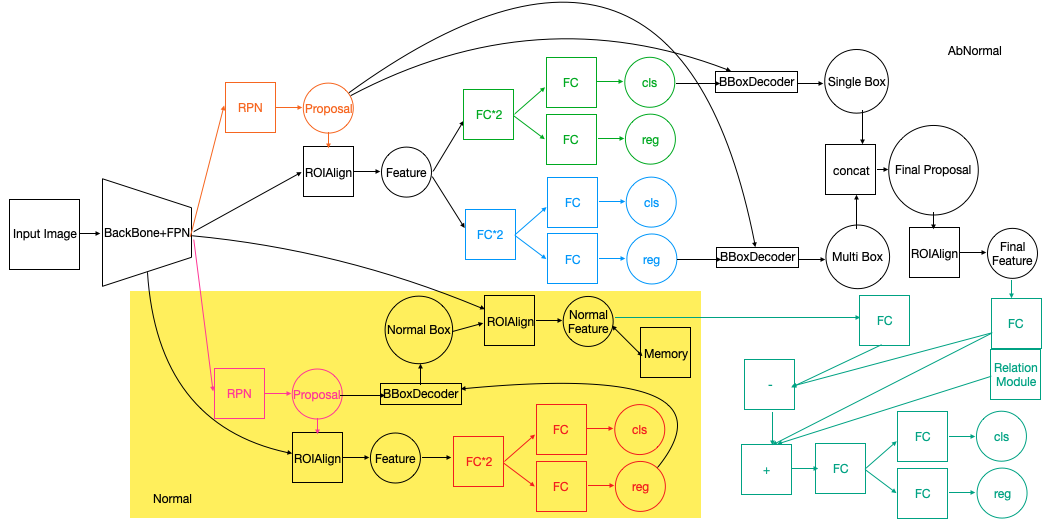
\includegraphics[width=0.6\paperwidth]{TCT/网络结构.png}
    \caption{模型的网络结构,图中ROIAlign指ROI层用于提取目标区域提案的特征,BBoxDecoder指预测框解码器,基于目标区域提案将模型的输出结果转化为预测框,Single Box和Multi Box指两个检测头的预测框,Normal box指检测到的正常细胞的标注框,Memory指正常细胞检测部分所使用的储存器,fc指全连接层,cls和reg分别指检测头的分类结果和回归结果}
    \label{pic:网络结构}
\end{figure}

\subsection{任务分解}
\label{sec:任务分解}
\subsubsection{标注框分解}
\label{sec:标注框分解}
\par 我们针对数据集中的每个病变细胞标注框,根据其中是否含有两个及以上的细胞,将其重新划分为病变种类-Single或病变种类-Multi类别。例如,一个LSIL的标注框内如果只有一个细胞,那么这个标注框将会被更改为LSIL-Single类别,反之,如果该标注框内含有两个及以上的细胞,那么这个标注框将会被更改为LSIL-Multi类别,如图\ref{pic:标注框分解}所示。而在训练时我们的数据集不仅仅会提供一份更改之前的标注框,还会分别提供仅含有Single类别和仅含有Multi类别的标注框,用于不同的检测头计算损失。
\begin{figure}[h]
    \centering
    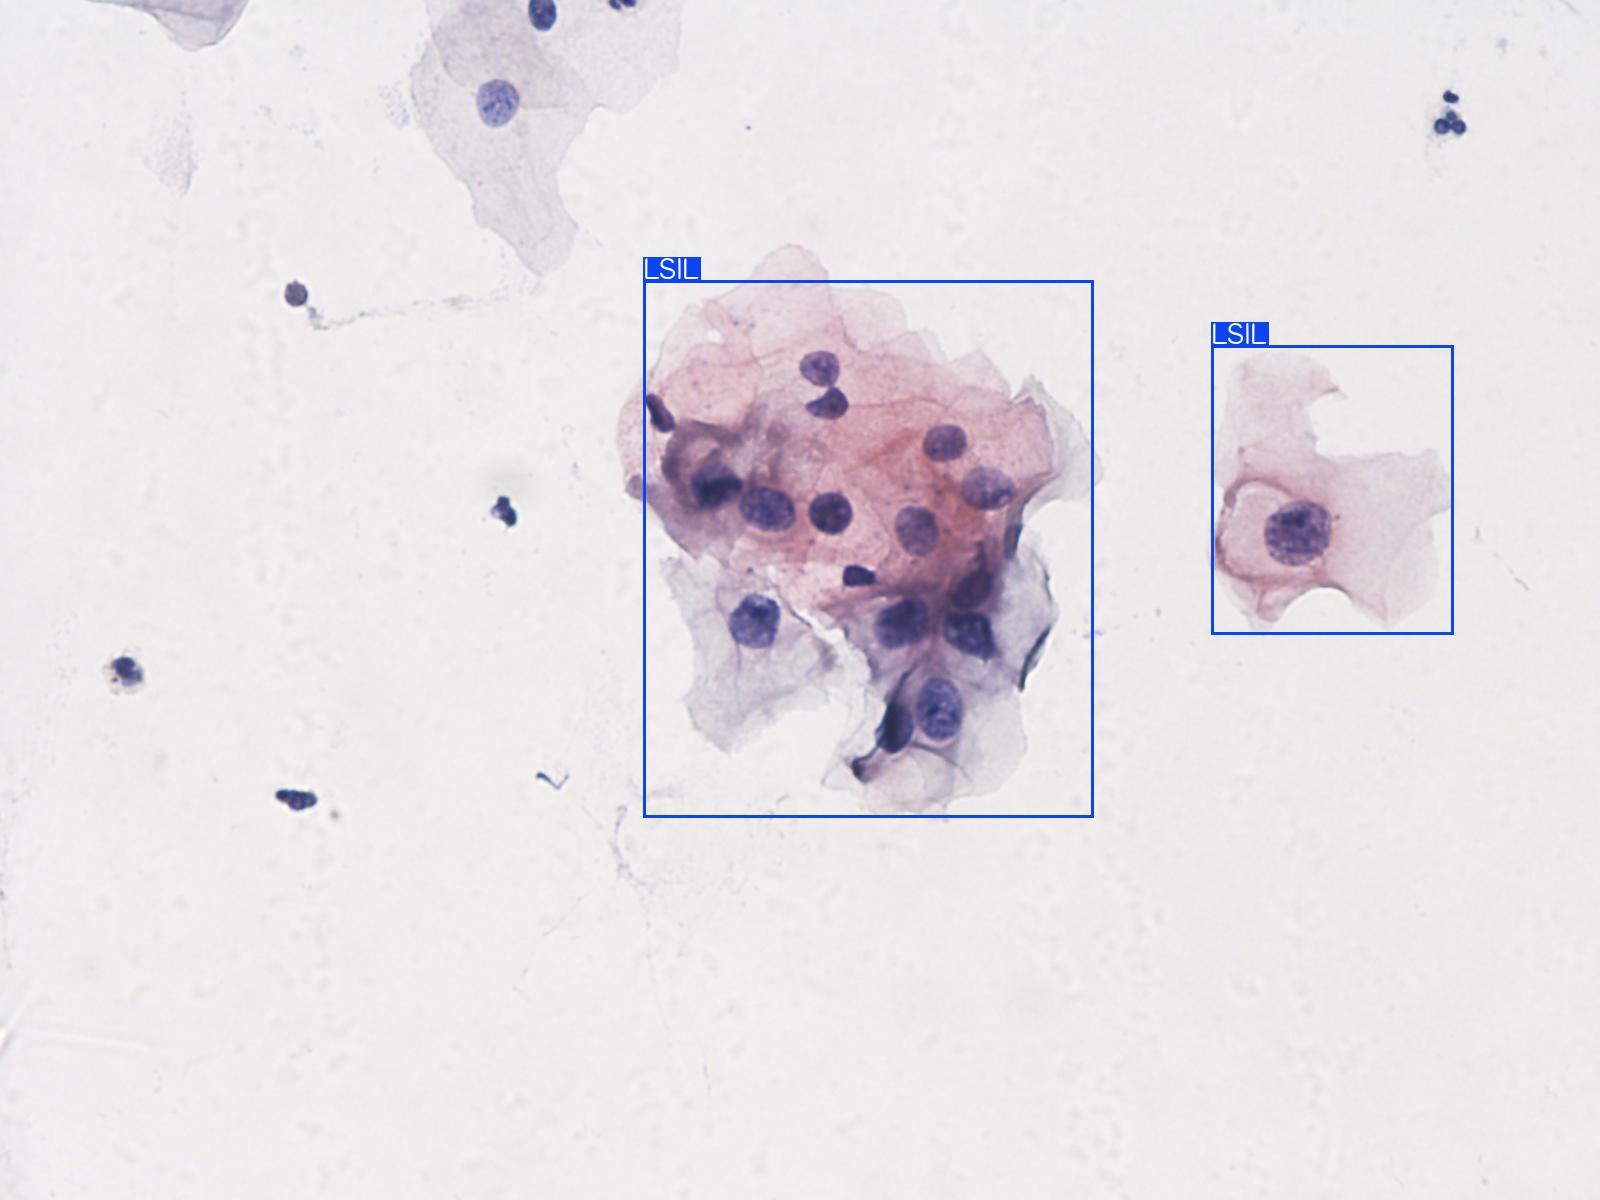
\includegraphics[width=0.6\paperwidth]{TCT/标注框分解.jpg}
    \caption{标注框分解示例,图中中间LSIL标注框中为一个细胞簇,含有两个以上的细胞将会被更改为LSIL-Multi标签,右侧LSIL标注框中为单个的细胞,将会被更改为LSIL-Single标签}
    \label{pic:标注框分解}
\end{figure}

\subsubsection{网络结构分离}
\par 网络结构分离部分主要对应图\ref{pic:网络结构}中间偏上部分的绿色和蓝色两个检测头,这两个检测头分别对应我们标注框分解\ref{sec:标注框分解}部分将标注框划分成的Singl和Multi类。在模型运行的过程中,我们的模型与Faster R-CNN模型一样也会首先使用Backbone和FPN层提取整张图片的特征,随后由一个RPN网络提出可能存在潜在目标的目标区域提案,之后这些目标区域提案将由ROI层提取相应的特征以获取这些区域所对应的特征图,最后这些特征图会被送入这两个检测头用于异常细胞的检测。
\par 正如我们在章节\ref{par:单细胞与细胞簇的形态差异}中所提到的,医生在标注框的时候会遇到大片病变细胞粘连在一起因而无法区分开的情况,这时医生只能选择将整个细胞簇框住,因此,每个标注框就有了两个可能的含义——单个病变细胞或者整个的病变细胞簇,而这二者有着明显的形态差异与语义差异,因此,我们为这两种不同的任务设计了不同的检测头,通过让每个检测头分别检测不同的目标达到提高检测准确度的目的。最后,我们会使用额外的一个检测头综合前面两个检测头的检测结果并给出最终结果,这样的设计既让不同的网络部分分别完成不同的任务,减轻了网络学习的负担,提高了网络的检测精度,又可以充分的利用到整张图像上的整体信息,不会造成由于信息的缺失而导致的性能下降等问题。
\par 在网络中,当RPN输出的目标区域提案经过ROI层提取出相应的特征之后,这些特征会分别被送入两个相互独立的检测头,这两个检测头的网络结构与Faster R-CNN中的检测头结构完全相同,都会让特征经过两个共享的全连接层之后再分别经过专门用于分类和回归的两个单独的全连接层完成整个检测头的预测过程。这两个检测头唯一的区别就是在训练的过程中,两个检测头输入的标注框不同。第一个检测头只会接受到仅含有单个细胞的标注框,而第二个检测头则恰恰相反,它只会接受到含有两个及以上细胞的标注框。
\par 特征图经过上述的两个检测头之后我们会分别获得两个分类结果和回归结果,我们会首先根据一定阈值刷选出分类结果达到该阈值的预测框,然后使用得到的回归结果计算出对应的预测框。检测头输出的回归结果是基于目标区域提案的一个偏移量$\Delta$,这种偏移量所对应的预测框满足公式\ref{eq:预测框偏移量}。其中,元组$(P_x, P_y, P_w, P_h)$是我们需要的预测框,元组$(R_x, R_y, R_w, R_h)$是RPN输出的目标区域提案,元组$(\Delta_x, \Delta_y, \Delta_w, \Delta_h)$是模型输出的回归结果。预测框和目标区域提案元组都是以xywh形式表达的框。其中,xy位置表示框的中心点座标,wh是框的宽和高,它们都经过了归一化,也即将相应的绝对大小除以了当前图片的宽和高以统一到0到1区间内。例如,在一个宽和高是$(2000, 1000)$的图片上,中心点为$(300, 500)$,宽和高分别是$(100,150)$的框在归一化之后所对应的元组应该是$(300, 500, 100, 150) / (2000, 1000, 2000, 1000) = (0.15, 0.5, 0.05, 0.15)$
\begin{equation}
    \begin{aligned}
        P_x & = R_W * \Delta_x + R_x \\
        P_y & = R_H * \Delta_y + R_y \\
        P_w & = R_W * e^{\Delta_w}   \\
        P_h & = R_H * e^{\Delta_h}   \\
    \end{aligned}
    \label{eq:预测框偏移量}
\end{equation}
\par 因此,当我们取得了两个检测头的预测结果之后,我们需要先通过公式\ref{eq:预测框偏移量}和目标区域提案计算出对应的预测框,再将两个结果直接拼接起来当作最终的检测头的目标区域提案。然后,我们最终的检测头就会基于这个拼接结果也即前两个检测头的预测框进行预测。在网络中,我们依然需要先通过ROI层提取出这些目标区域提案的特征,之后我们会将这些特征过一个单独的全连接层当作异常细胞的特征,同时,我们也会将正常细胞检测部分获得的正常细胞的特征也过一个单独的全连接层,作为正常细胞的特征。我们会使用一个经过单独设计的关系计算模块计算出异常细胞之间的关系特征,也会通过异常细胞特征与正常细胞特征直接做差计算出异常细胞与正常细胞之间的差分特征,最后我们会将异常细胞的特征与关系特征、差分特征直接加和送入之后的检测头中进行检测。具体来说,我们会将最终得到的特征经过一层共享的全连接层,再经过专门用于分类和回归的两个单独的全连接层完成预测过程。

\subsection{细胞对比}
\par 医生在为标注框标注类别时可能会有较大的主观倾向性,而且由于病变是一个不断发展的过程,病变细胞在不断发展的过程中可能会刚好处于某两个类别之间的状况,这时的病变细胞会同时具有这两个类别的某些特征,这就会影响医生对细胞类别的判断,也会造成病变类别判断的模糊性与不明确性。因此,如何准确的判断检测到的病变细胞的类别是一个较大的困难,我们为此设计了多个模块帮助网络加强对病变细胞类别的判断。

\subsubsection{半监督学习与伪标签的生成}
\label{半监督学习与伪标签的生成}
\par 在特征差分模块中我们需要使用正常细胞的特征,然而,在实际检测的过程和临床上,医生一般只会对病变细胞给出病变区域的标注,而对于正常细胞医生只会自己在片子中观察到正常细胞后用于辅助诊断,但不会在诊断结果中注明。因此,我们希望能让模型尽可能少的使用“额外的”正常细胞的标注以减少这个过程会增加的工作量。为此,我们首先将数据集中正常细胞的标注看作全部正常细胞标注的一个真子集,让模型在初始的数据集上先训练一轮,然后通过验证集验证后取得在验证集上表现较好的模型,再使用这个模型为整个数据集全部预测一次,将预测结果用一个固定的分数阈值过滤后与原来的标注框计算iou,除去iou过高的预测框后,将剩余的所有预测框加入到标注框中。最后不断的重复这个过程,让模型不断迭代最终获得客观上全部的正常细胞的标注。
\par 另一方面,我们希望探究启动如上机制至少需要多少正常细胞的标注。为此,我们首先标注了大量的正常细胞,并通过使用不同比例的正常细胞标注来作为初始数据集完成上述的迭代过程训练模型以找到最低限度正常细胞标注数量。
\par 我们使用从1\%到100\%总计八种不同的比例来启动实验以测试不同数量的正常细胞标注是否能够正常启动上述机制以达到让模型在只有少量正常细胞标注的情况下完成正常细胞检测工作的任务。各种比例下的正常细胞标注框数量与对应图片数量如表\ref{tab:正常细胞数量}所示。

\begin{table}[htbp]
    \center
    \caption{各类别标注框数量与图片数量}
    \begin{tabular}{ccccccccc}
        \hline
        比例       & 1\% & 3\% & 5\% & 10\% & 25\% & 50\% & 75\% & 100\% \\
        \hline
        标注框数量 & 29  & 87  & 145 & 290  & 723  & 1446 & 2169 & 2891  \\
        图片数量   & 29  & 86  & 140 & 280  & 637  & 1102 & 1475 & 1739  \\
        \hline
    \end{tabular}
    \label{tab:正常细胞数量}
\end{table}
结果如\ref{tab:正常细胞半监督检测}所示,可以看到,即便只使用我们认为只需要至少量的标注框(五十到一百五十)就可以通过上述机制完成模型对检测正常细胞任务的学习。
\subsubsection{正常细胞检测}
\par 在细胞对比的过程中,我们需要用到同一张图像上的正常细胞的特征,因此,我们的模型除了要能够成功地捕捉到异常细胞特征以外,还要能够捕捉到正常细胞的特征。
\par 正常细胞检测部分对应图\ref{pic:网络结构}左下角黄色背景部分,我们模型对于正常细胞的检测部分完全使用了Faster R-CNN的结构,首先图片会经过Backbone和FPN提取特征。正常细胞检测部分所使用的Backbone和FPN层是与异常细胞检测部分共用的,这样的设计既能大幅降低模型的参数量便于训练和部署,又可以让Backbone和FPN层在同样数量的训练集下获得更多的梯度更新,有助于模型的训练和学习。然后再使用一个RPN模块提取潜在的目标区域提案,需要注意的是,这个RPN模块与异常细胞部分所使用的RPN模块是分离的,两部分不共享权重,这样的设计可以让两个RPN模块分别专注于检测正常细胞与异常细胞,避免模型在训练和学习的过程中遇到特征冲突和语义冲突等情况。之后我们会将RPN模块提取出的目标区域提案使用ROI层提取出对应的特征图,然后这些特征图会经过两个共享的全连接层,再经过专门用于分类和回归的两个单独的全连接层完成正常细胞检测部分的预测过程。
\par 与异常细胞检测部分一样,正常细胞检测部分的回归预测结果也是基于目标区域提案的偏移量,因此,当我们正常细胞检测部分结束之后,我们首先需要根据模型预测的分类结果对每张图选出得分最高的预测结果,再根据公式\ref{eq:预测框偏移量}和目标区域提案计算出对应的预测框。之后我们会将预测出来的正常细胞的结果送入ROI层进行提取特征,再将提取出来的正常细胞的特征送入模型的储存器中储存起来,当我们没有从某张图片中检测出正常细胞时,我们就会从改储存器中随机挑选一个正常细胞的特征当作当前图片中检测出来的正常细胞的特征来使用,而如果存储器中也没有储存着正常细胞的特征,那么我们会用一个全零的张量作为正常细胞的特征。

\subsubsection{细胞对比模块}
\paragraph{正常细胞与异常细胞对比}
\label{sec:正常细胞与异常细胞对比}
\par 我们使用特征差分模块进行正常细胞与异常细胞的对比,该模块对应图\ref{pic:网络结构}右下角深绿色的减号,它会使用当前图片中所有的检测到的病变细胞的特征以及我们前面获得的当前图片或从存储器中随机挑选出来的正常细胞的特征直接做减法得到异常细胞与正常细胞之间的差分特征。首先,我们会现将正常细胞的特征重复多次,复制到与异常细胞的特征同样的尺寸。然后,我们会直接用异常细胞的特征减去正常细胞的特征获得异常细胞与正常细胞之间的差分特征。如公式\ref{eq:差分计算}所示。其中,$F_A$是指所有病变细胞的特征,$F_N$是指所使用的正常细胞的特征,$F_D$表示计算得到的差分特征。

\begin{equation}
    \begin{aligned}
        F_D & =F_A-F_N
    \end{aligned}
    \label{eq:差分计算}
\end{equation}

\paragraph{异常细胞与异常细胞对比}
\label{sec:异常细胞与异常细胞对比}
\par 我们使用病变细胞关系模块进行异常细胞与异常细胞之间的对比,这一模块对应图\ref{pic:网络结构}右下角深绿色的Relation Module,它会将当前图片中所有的检测到的病变细胞的特征计算一次两两之间的关系,并得到新的关系特征,如公式\ref{eq:关系计算}所示。其中,$F$是指病变细胞的特征,它是图\ref{pic:网络结构}中的Final Feature,由前两个检测头预测出的预测框提特征得到,是一个$N\times M$的矩阵,其中,$N$是当前图片中检测到的病变细胞的数量,$M$是每个病变细胞特征的维度,在本文中我们取$1024$。$P$是一个$M\times M$的矩阵,它表示将病变细胞的特征转化到某个编码空间中的编码方式,是一个可学习的参数。$W_R$表示病变细胞特征之间的关系权重。$F_R$表示计算得到的关系特征。

\begin{equation}
    \begin{aligned}
        W_R & =Softmax((FP)(FP)^T) \\
        F_R & =W_RF
    \end{aligned}
    \label{eq:关系计算}
\end{equation}

\par 而上述关系计算的过程中,每两个特征之间的关系仅是关系权重矩阵中的一个数字,这可能不足以表达特征之间的关系。因此,我们设计了分区的病变细胞关系模块。这一模块首先将病变细胞特征进行分区,例如病变细胞的特征是$N\times 1024$的一个矩阵,其中$N$表示病变细胞特征的数量。我们如果要分为$8$个区的话,我们就会得到一个$N\times 8 \times 128$的一个张量,然后我们通过转置可以获得一个$8\times N\times 128$的张量,这时,我们需要使用的可学习的变换矩阵会是$8\times 128 \times 128$的一个张量,那么公式\ref{eq:关系计算}就会变为

\begin{equation}
    \begin{aligned}
        W_R & =Softmax((F\otimes P)(F\otimes P)^T) \\
        F_R & =W_R\otimes F
    \end{aligned}
    \label{eq:分区版关系计算}
\end{equation}

\par 其中,$\otimes$是指按批次的矩阵乘法,$M\otimes N$相当于将两个三维张量$M$和$N$看作矩阵的列表,将$M$和$N$中的每一个矩阵依次做矩阵乘法并将结果拼接起来重新变为一个三维张量。$F$、$P$的含义与之前相同,不过都是张量的表达形式。计算得到$F_R$也是一个三维张量,需要先通过转置和变形,变回二维矩阵形式。

\paragraph{综合}
\par 当我们完成所有的特征计算之后我们会直接将关系特征、差分特征与初始的病变细胞的特征直接相加用作之后的检测,这部份对应图\ref{pic:网络结构}右下角深绿色的加号,其使用的公式如\ref{eq:特征融合}所示。其中,$F_F$是指最后计算得到的特征,$F$是指初始的病变细胞的特征,$F_R$是指关系计算得到的特征,$F_R$是指差分计算得到的特征。

\begin{equation}
    \begin{aligned}
        F_F & =F+F_R+F_D
    \end{aligned}
    \label{eq:特征融合}
\end{equation}

\clearpage

\section{实验与结果}

\subsection{数据集}
\subsubsection{数据集总览}
\par 我们的数据集拥有6957张图片,包含ASCUS(非典型鳞状细胞意义不明确)、LSIL(低度鳞状上皮内病变)、ASCH(非典型鳞状细胞不排除高级别鳞状上皮内病变)、HSIL(高度鳞状上皮内病变)、SQCA(鳞状上皮癌)五种病变类别,以及NORMAL(正常细胞)一种正常类别。其中,图片中所有的这五种类别的病变细胞几乎已经被完全标注,可以认为除去标注框所标注的这五种病变细胞以外,数据集中不含有其他属于该五种病变的细胞。但是,正常细胞由于数量过多,实践中也不可能将视野中的正常细胞全部标注等问题,数据集仅注明了视野中的一部分正常细胞。各类别标注框的数量与含有该类别的图片的数量如表\ref{tab:类别}所示。

\begin{table}[htbp]
    \center
    \caption{各类别标注框数量与图片数量}
    \begin{tabular}{cccc}
        \hline
        类别   & 标注框数量 & 图片数量 \\
        \hline
        ASCH   & 1357       & 946      \\
        ASCUS  & 4065       & 2635     \\
        HSIL   & 13001      & 2771     \\
        LSIL   & 3241       & 2323     \\
        SQCA   & 390        & 124      \\
        NORMAL & 4796       & 2872     \\
        TOTAL  & 22054      & 6935     \\
        \hline
    \end{tabular}
    \label{tab:类别}
\end{table}

\par 此外,我们的数据集中的图片拥有不同的放大倍率以及图片尺寸,其中,图片的尺寸以$1024*768$的图片最多,$744*554$的图片只有一张最少。详细数量如表\ref{tab:尺寸}所示。

\begin{table}[htbp]
    \center
    \caption{各类别标注框数量与图片数量}
    \begin{tabular}{cccc}
        \hline
        图片的长 & 图片的宽 & 图片数量 \\
        \hline
        1024     & 768      & 3206     \\
        2048     & 1536     & 1986     \\
        768      & 576      & 973      \\
        1600     & 1200     & 750      \\
        640      & 480      & 31       \\
        1280     & 960      & 10       \\
        744      & 554      & 1        \\
        \hline
    \end{tabular}
    \label{tab:尺寸}
\end{table}

部分数据集中图片与标注框的可视化如图\ref{pic:数据集可视化}所示。
\begin{figure}[htb]
    \centering
    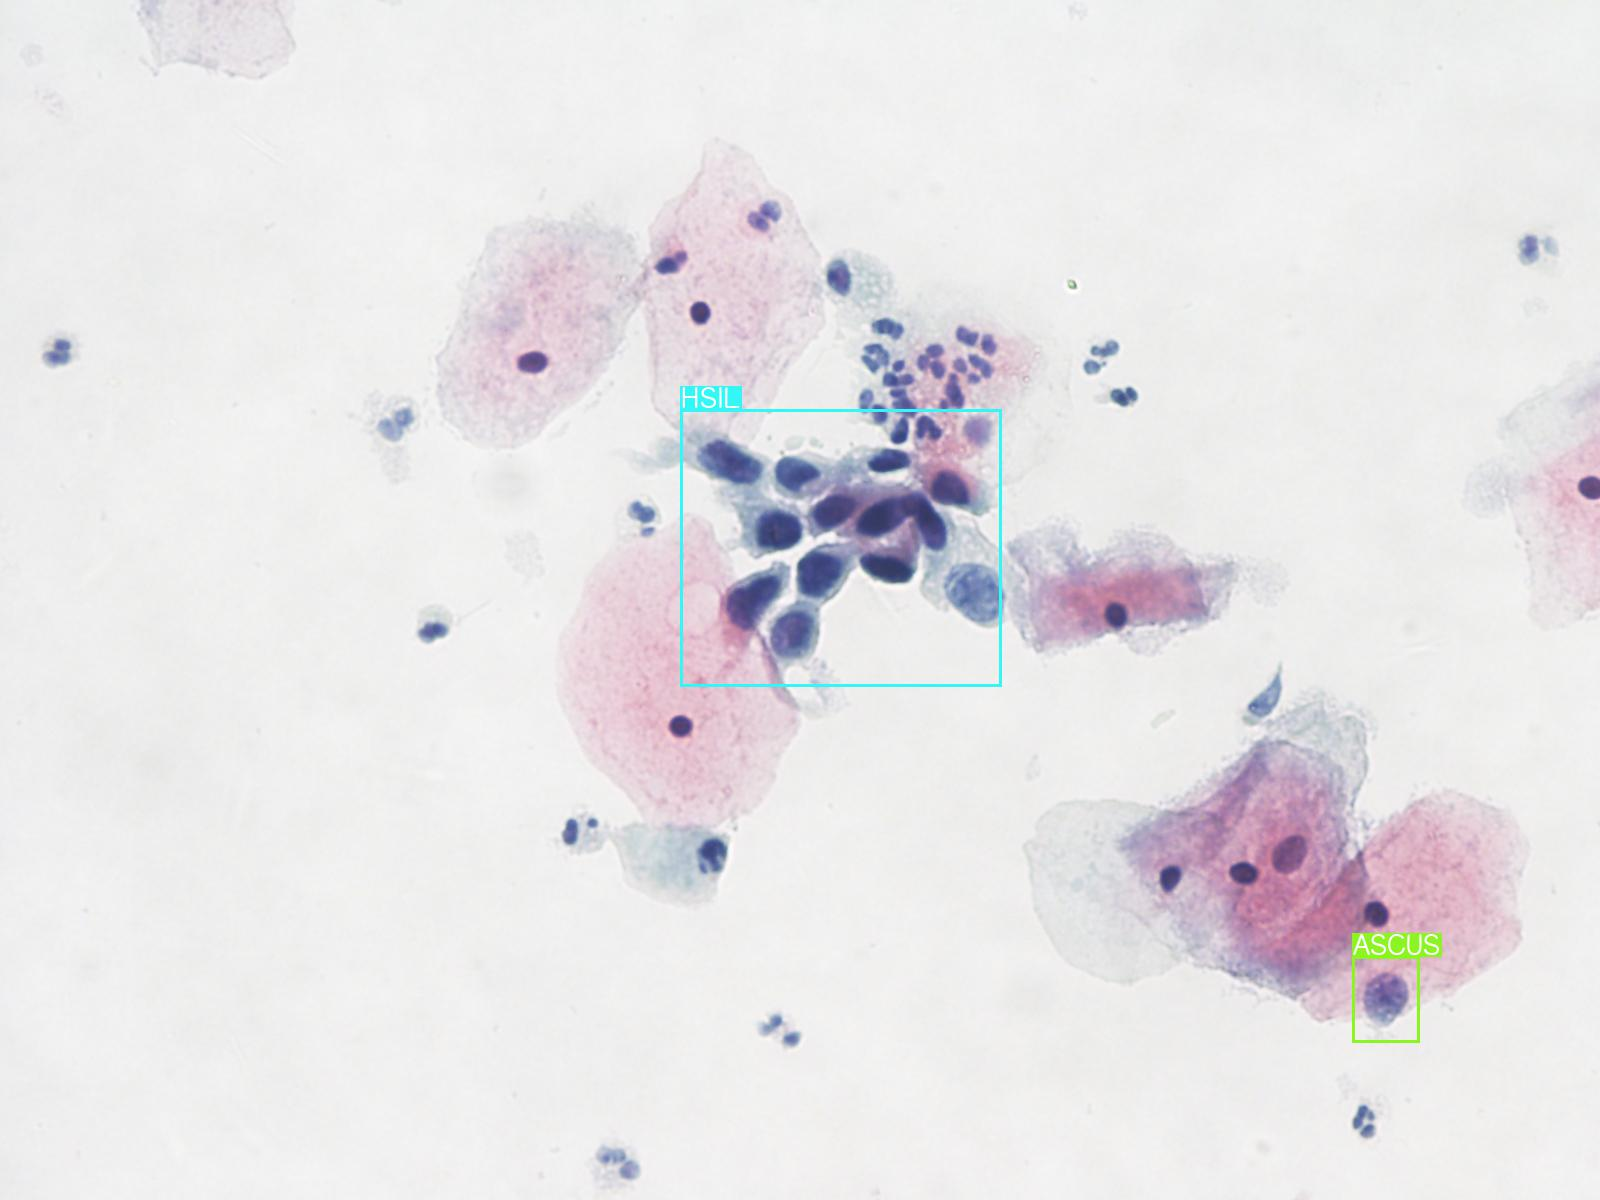
\includegraphics[width = .49\linewidth]{TCTDataSet/可视化1.jpg}
    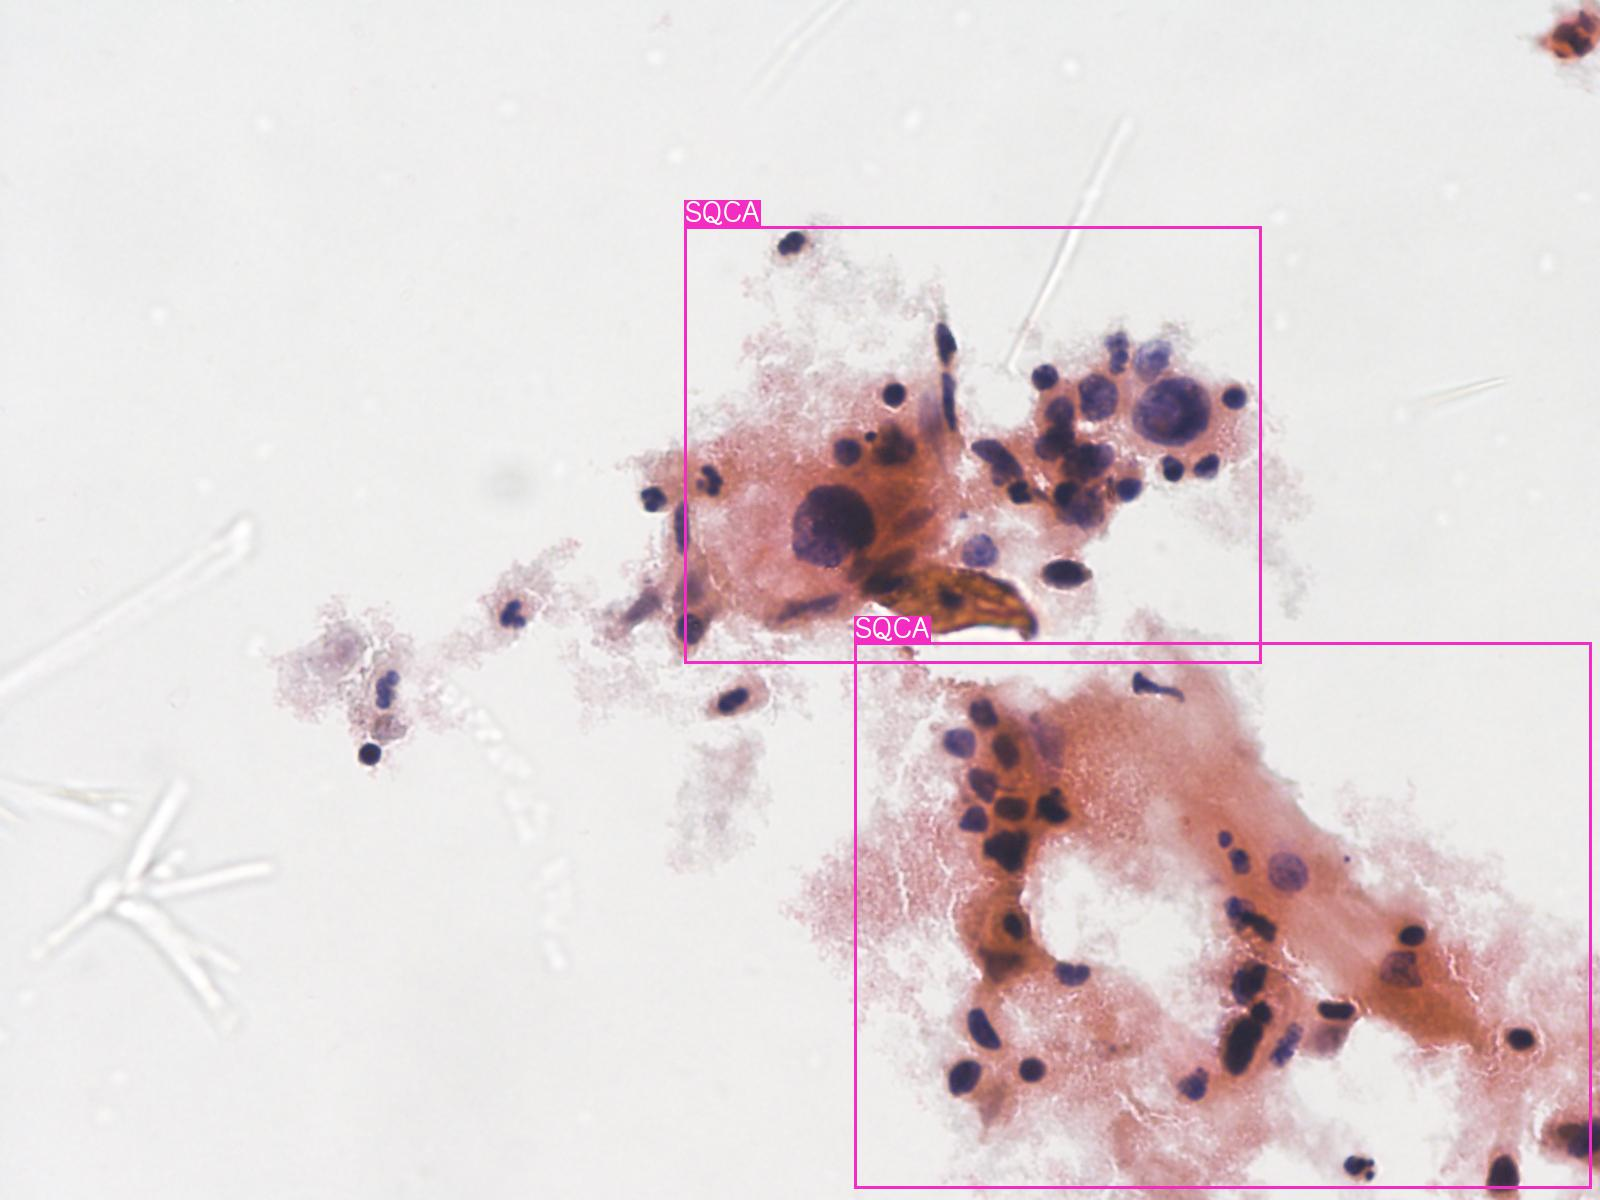
\includegraphics[width = .49\linewidth]{TCTDataSet/可视化2.jpg}
    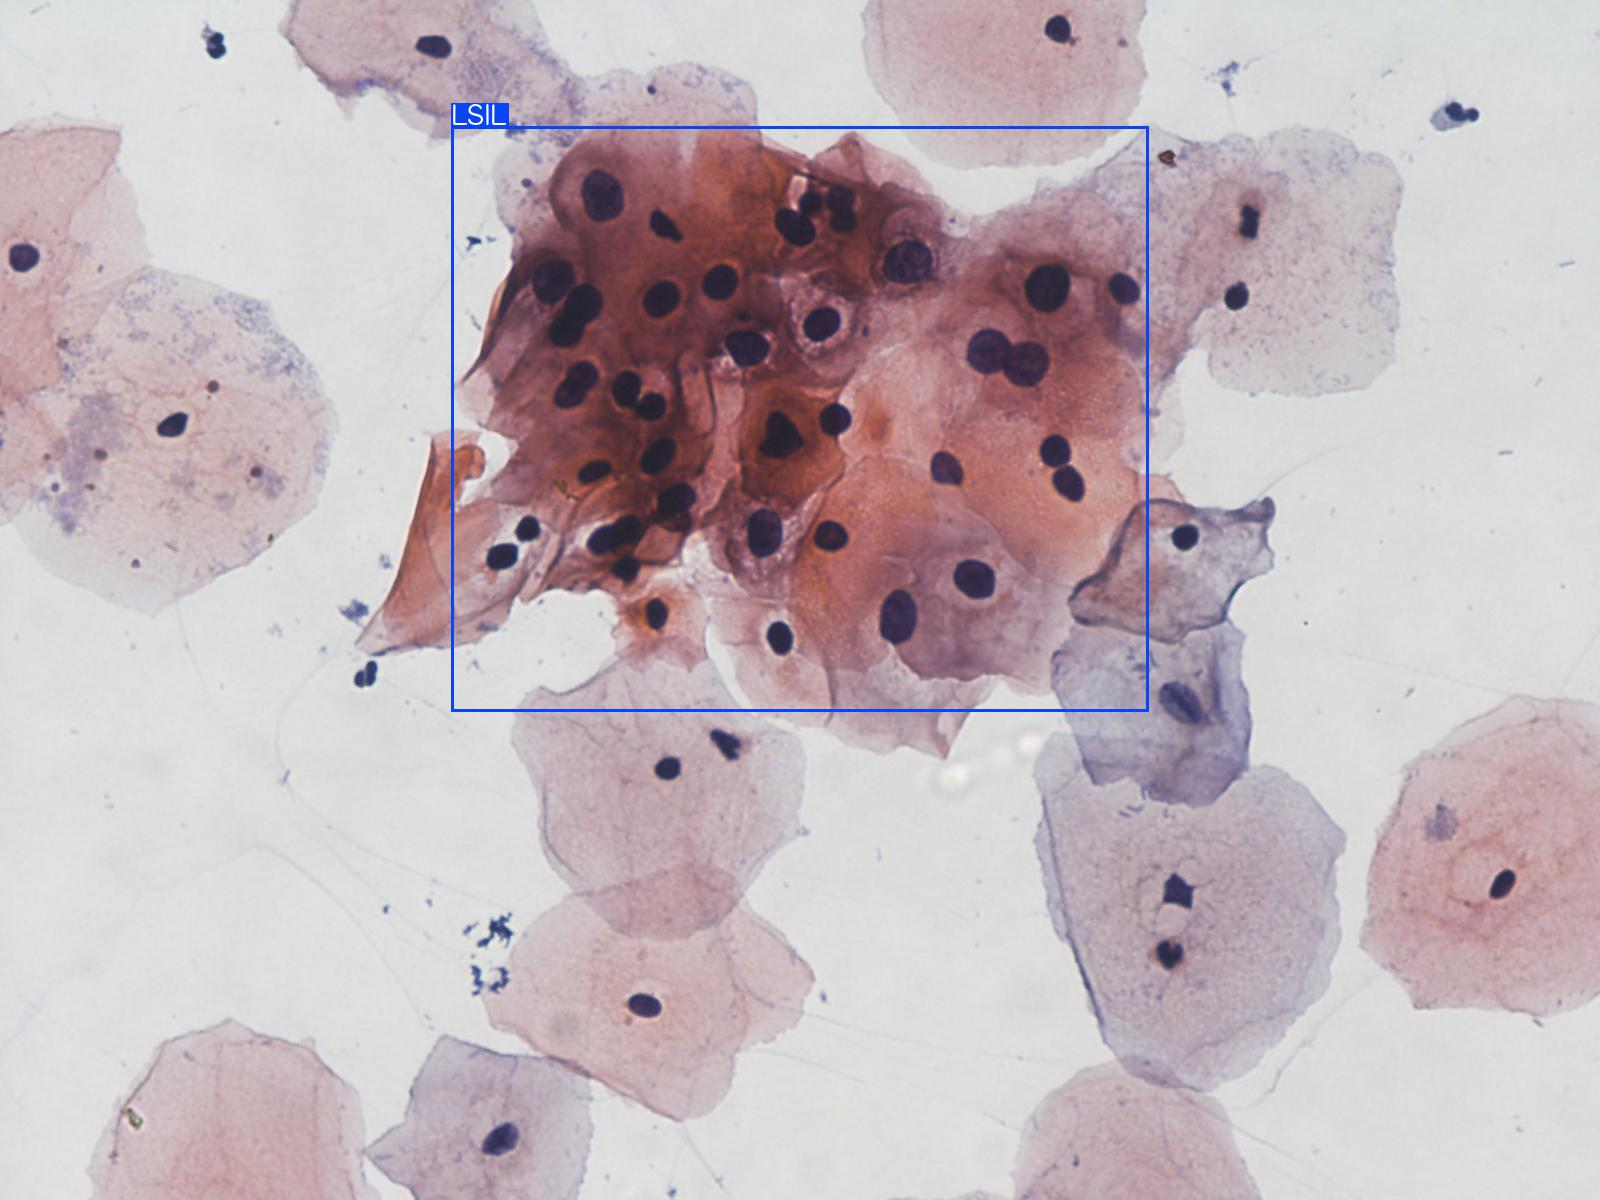
\includegraphics[width = .49\linewidth]{TCTDataSet/可视化3.jpg}
    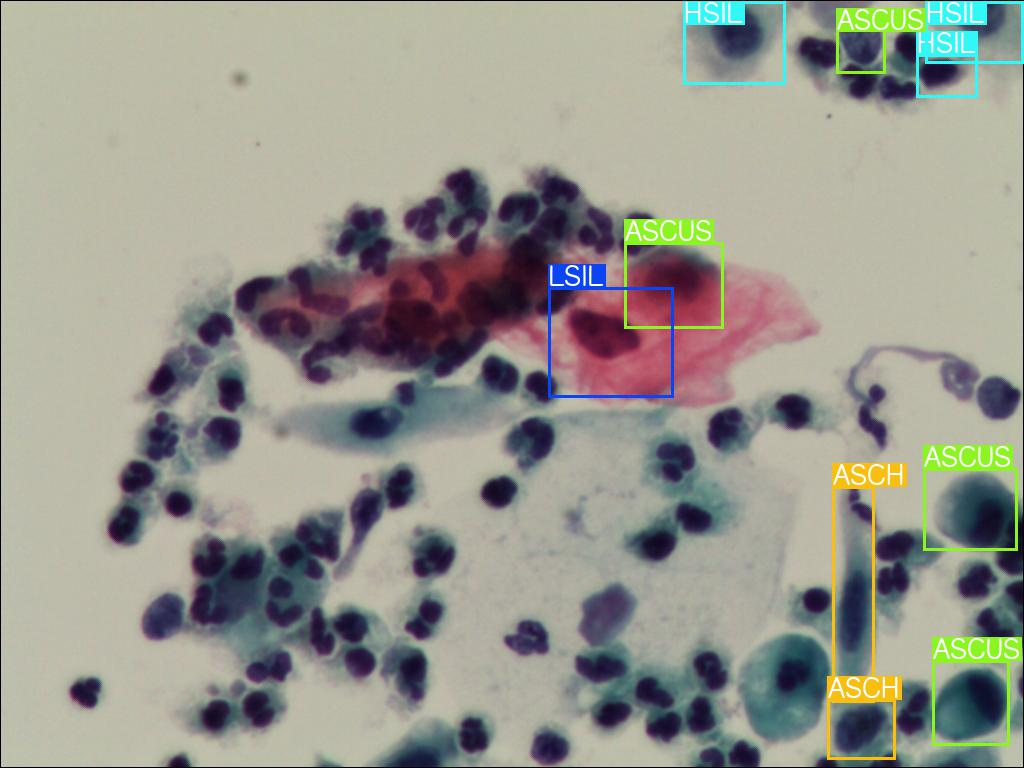
\includegraphics[width = .49\linewidth]{TCTDataSet/可视化4.jpg}
    \caption{部分数据集图片和标注框的可视化结果}
    \label{pic:数据集可视化}
\end{figure}

\subsubsection{数据集划分}
\par 我们将整个的数据集按照$6:2:2$的比例划分为训练集、验证集和测试集。其中,训练集主要用来训练模型,对于模型需要用到的多个超参数,我们会在训练集上尝试超参数的不同组合方式并在验证集上验证不同超参数组合下的模型的预测结果,从这其中选取出在验证集上效果最优的模型作为该模型的最优权重。最后将使用这一最优的权重在测试集上进行测试以获取该模型在测试集上的结果,并将这一结果作为当前模型在实际预测过程中的检测结果。
\par 训练集、验证集和测试集三个数据集上各个类别的标注数量如表\ref{tab:各数据集类别}所示。其中,TOTAL的标注框数量指的是除去NORMAL类别以外,所有病变细胞类别所有标注框数量的总和。TOTAL的图片数量是指该数据集所拥有的所有图片的数量。

\begin{table}[htbp]
    \center
    \caption{各数据集上不同类别标注框数量与图片数量}
    \begin{tabular}{ccccccc}
        \hline
               & 训练集     &          & 验证集     &          & 测试集     &          \\
        类别   & 标注框数量 & 图片数量 & 标注框数量 & 图片数量 & 标注框数量 & 图片数量 \\
        \hline
        ASCH   & 786        & 553      & 291        & 203      & 280        & 190      \\
        ASCUS  & 2363       & 1571     & 849        & 549      & 853        & 515      \\
        HSIL   & 7972       & 1673     & 2411       & 528      & 2618       & 570      \\
        LSIL   & 1929       & 1415     & 657        & 455      & 655        & 453      \\
        SQCA   & 241        & 71       & 68         & 25       & 81         & 28       \\
        NORMAL & 2891       & 1739     & 936        & 559      & 969        & 574      \\
        TOTAL  & 13291      & 4159     & 4276       & 1389     & 4487       & 1387     \\
        \hline
    \end{tabular}
    \label{tab:各数据集类别}
\end{table}

\subsection{数据预处理与数据增强}
\paragraph{放缩}
\par 我们首先将图片保持宽高比地放缩到不大于宽1333个像素,高800个像素的最大尺寸,例如,如果一张图片的大小是宽1024个像素,高720个像素,那么,如果将宽放大到1333个像素则会放大大约$1.3$倍,而如果将高放大到800个像素则会放大大约$1.11$倍,而$1.3>1.11$,因此,图片只能将高放大到800个像素,宽度放大到1138个像素。这样既保持了图片的宽高比没有被改变从而没有使图片变形,又保证了图片不会超过预设的尺寸因而可以被放入网络中进行计算。
\paragraph{随机翻转}
\par 当我们每次从数据集中取出一张图片时,我们会有$50\%$的概率将这张图片进行水平的翻转,而另有$50\%$的概率将直接读取这张图片不做任何变化。
\paragraph{正规化}
\par 我们会将数据集中的每张图片都做正规化处理再进行训练,这是指将图片中的每个像素的三个通道都减去平均值再除以相应的标准差,如公式\ref{eq:正规化预处理}所示。
\begin{equation}
    P_{i,j,c}=\frac{P_{i,j,c}-mean_{c}}{std_{c}}
    \label{eq:正规化预处理}
\end{equation}

\par 其中,$P_{i,j,c}$是指图片在$i,j$处$c$通道的值,$mean$和$std$都是三维的向量,分别表示三个通道在整个数据集上的平均值与标准差,其计算方式如公式\ref{eq:正规化参数}所示。
\begin{equation}
    \begin{aligned}
        mean_c & =\frac{\sum_{k=0}^N\frac{\sum_{i=0}^{H^k}\sum_{j=0}^{W^k}P_{i,j,c}^k}{H^k*W^k}}{N}                   \\
        std_c  & =\sqrt{\frac{\sum_{k=0}^N\frac{\sum_{i=0}^{H^k}\sum_{j=0}^{W^k}(P_{i,j,c}^k-mean_c)^2}{H^k*W^k}}{N}}
    \end{aligned}
    \label{eq:正规化参数}
\end{equation}

\par 其中,$P_{i,j,c}^k$是指数据集中的第k张图片在$i,j$处$c$通道的值,$H^K$和$W^k$分别指第k张图片的高和宽,$N$是指数据集中共有$N$张图片。在本文中,$mean$与$std$变量的取值如\ref{eq:正规化参数取值}所示。
\begin{equation}
    \begin{aligned}
        mean & =[123.675, 116.28, 103.53] \\
        std  & =[58.395, 57.12, 57.375]
    \end{aligned}
    \label{eq:正规化参数取值}
\end{equation}

\subsection{实现细节}
\par 我们使用mmdetection\cite{chen2019mmdetection}框架完成整个模型的设计和实验过程,我们的模型最终运行在一台拥有7张1080Ti显卡的Ubuntu 16.04的服务器上,训练和测试过程中我们每个实验只会使用一张1080Ti显卡。在我们的训练过程中,我们使用了0.005的学习率训练了12个epoch,学习率将会在第8和第11个epoch时降低为之前的0.1倍。我们还使用了warm up策略,学习率会在前500个迭代内线性增大到0.005。我们使用SGD优化器并设置了0.9的momentum和0.0001的weight decay。

\subsection{评价指标}
\par 我们使用mAP作为评价模型的指标。而mAP的计算设计IOU、PR曲线以及AP等。

\paragraph{IOU}
\par IOU也即交并比是指两个矩形框交集的面积与并集的面积之比。它通常用来描述两个矩形框的相似性,两个矩形框的交并比越接近1就越相似,反之,越接近0就越不相似。

\paragraph{True Positive}
\par True Positive也即TP,指的是正确的预测结果,在目标检测领域是指与标注框的IOU大于IOU阈值的预测框的数量。类似的还有False Positive 也即FP,指的是错误的预测结果,也即与标注框的IOU小于等于IOU阈值的预测框的数量,False Negative 也即FN,指的是没有预测出来的标注框。

\paragraph{查准率与查全率}
\par 查准率也即Precision是TP与TP+FP的比值。也即
$$Precision=\frac{TP}{TP+FP}$$
\par 其中,在目标检测领域,TP+FP表示所有预测框的数量,也即
$$Precision=\frac{TP}{\text{number of detections}}$$
\par 查全率也即Recall是TP与TP+FN的比值。也即
$$Precision=\frac{TP}{TP+FN}$$
\par 其中,在目标检测领域,TP+FN表示所有标注框的数量,也即
$$Precision=\frac{TP}{\text{number of ground truths}}$$

\paragraph{PR曲线}
\par 首先我们需要将所有的预测框和标注框之间两两计算IOU,对于每一个标注框如果有预测框与当前标注框的IOU大于IOU阈值,那么该标注框就会选择IOU最高的一个预测框作为自己的分配结果,而如果没有预测框与当前标注框的IOU大于IOU阈值,那么当前的标注框就会被认为是没有被检测到成为一个FP。如果一个预测框被分配给了一个标注框,那么这个预测框就认为是正确的预测框,成为一个TP,反之,就会被认为是一个错误的预测成为一个FP。
\par 其次,我们需要知道当模型做出预测结果时,除去会输出一个四个元素的元组表示预测框以外,还会输出一个对该预测框的置信度。而我们如果把所有的预测框按照这个置信度进行降序排列就会得到一个预测框的队列。那么我们就可以按照这个队列的顺序计算当我们只从队列中取出前k个预测框时,对应的查准率和查全率,而如果我们把k从1取到这个队列的长度,我们就获得了多组(查准率,查全率)元组,按照这些元组绘制成的曲线就是PR曲线。

\paragraph{Average Precision}
\par Average Precision也即AP,指的是PR曲线下的面积。而在我们计算AP的时候,我们往往不会绘制无限精细的PR曲线用于计算AP,而是对于每一个查全率选取最高的查准率,而认为两个计算得到的查全率之间查准率不会发生变化,以此来计算AP值。

\paragraph{mean Average Precision}
\par mean Average Precision也即mAP,指的是各个类别AP的平均值。此外,由于AP的计算以及PR曲线的绘制需要用到IOU阈值,因此,mAP也会因为IOU阈值的不同而不同,本文中使用的mAP50和mAP75就是指IOU阈值为0.5和0.75时的mAP,而本文使用的mAP是指IOU阈值为0.5到0.95时的平均值。

\subsection{与其他相关工作的检测性能对比}
\par 如章节\ref{sec:国内外研究现状}所示,国内外已有许多关于宫颈病变细胞检测的工作和研究,还有许多目标检测方面的工作可以用于宫颈病变细胞的检测。我们选用了其中一部分具有代表性的工作和一些基线模型在我们的数据集上做了检测结果的对比,结果如\ref{tab:模型结果对比}所示。

\begin{table}[htbp]
    \centering
    \caption{模型结果对比}
    \begin{tabular}{|c|c|c|c|c|}
        \hline
        模型                       & 验证集mAP50   & mAP           & mAP50         & mAP75         \\ \hline
        \textbf{TCT-RCNN(ours)}    & \textbf{48.7} & \textbf{25.5} & \textbf{47.7} & \textbf{24.2} \\ \hline
        Faster-RCNN                & 46.0          & 23.8          & 47.3          & 20.4          \\ \hline
        Casacde-RCNN               & 44.9          & 25.4          & 46.1          & 26.0          \\ \hline
        Sparse-RCNN                & 39.0          & 20.0          & 37.0          & 19.7          \\ \hline
        Retinanet                  & 43.5          & 22.3          & 42.4          & 20.9          \\ \hline
        RepPoints                  & 46.3          & 24.2          & 45.4          & 23.8          \\ \hline
        YoloV3                     & 36.7          & 17.2          & 36.9          & 14.2          \\ \hline
        Comparison detector        & 14.2          & 2.9           & 7.7           & 1.4           \\ \hline
        Faster-RCNN VGG16 Backbone & 36.2          & 17.7          & 36.9          & 15.4          \\ \hline
    \end{tabular}
    \label{tab:模型结果对比}
\end{table}
\par 我们的模型部分检测结果的可视化如图\ref{pic:检测结果可视化}所示。
\begin{figure}[htb]
    \centering
    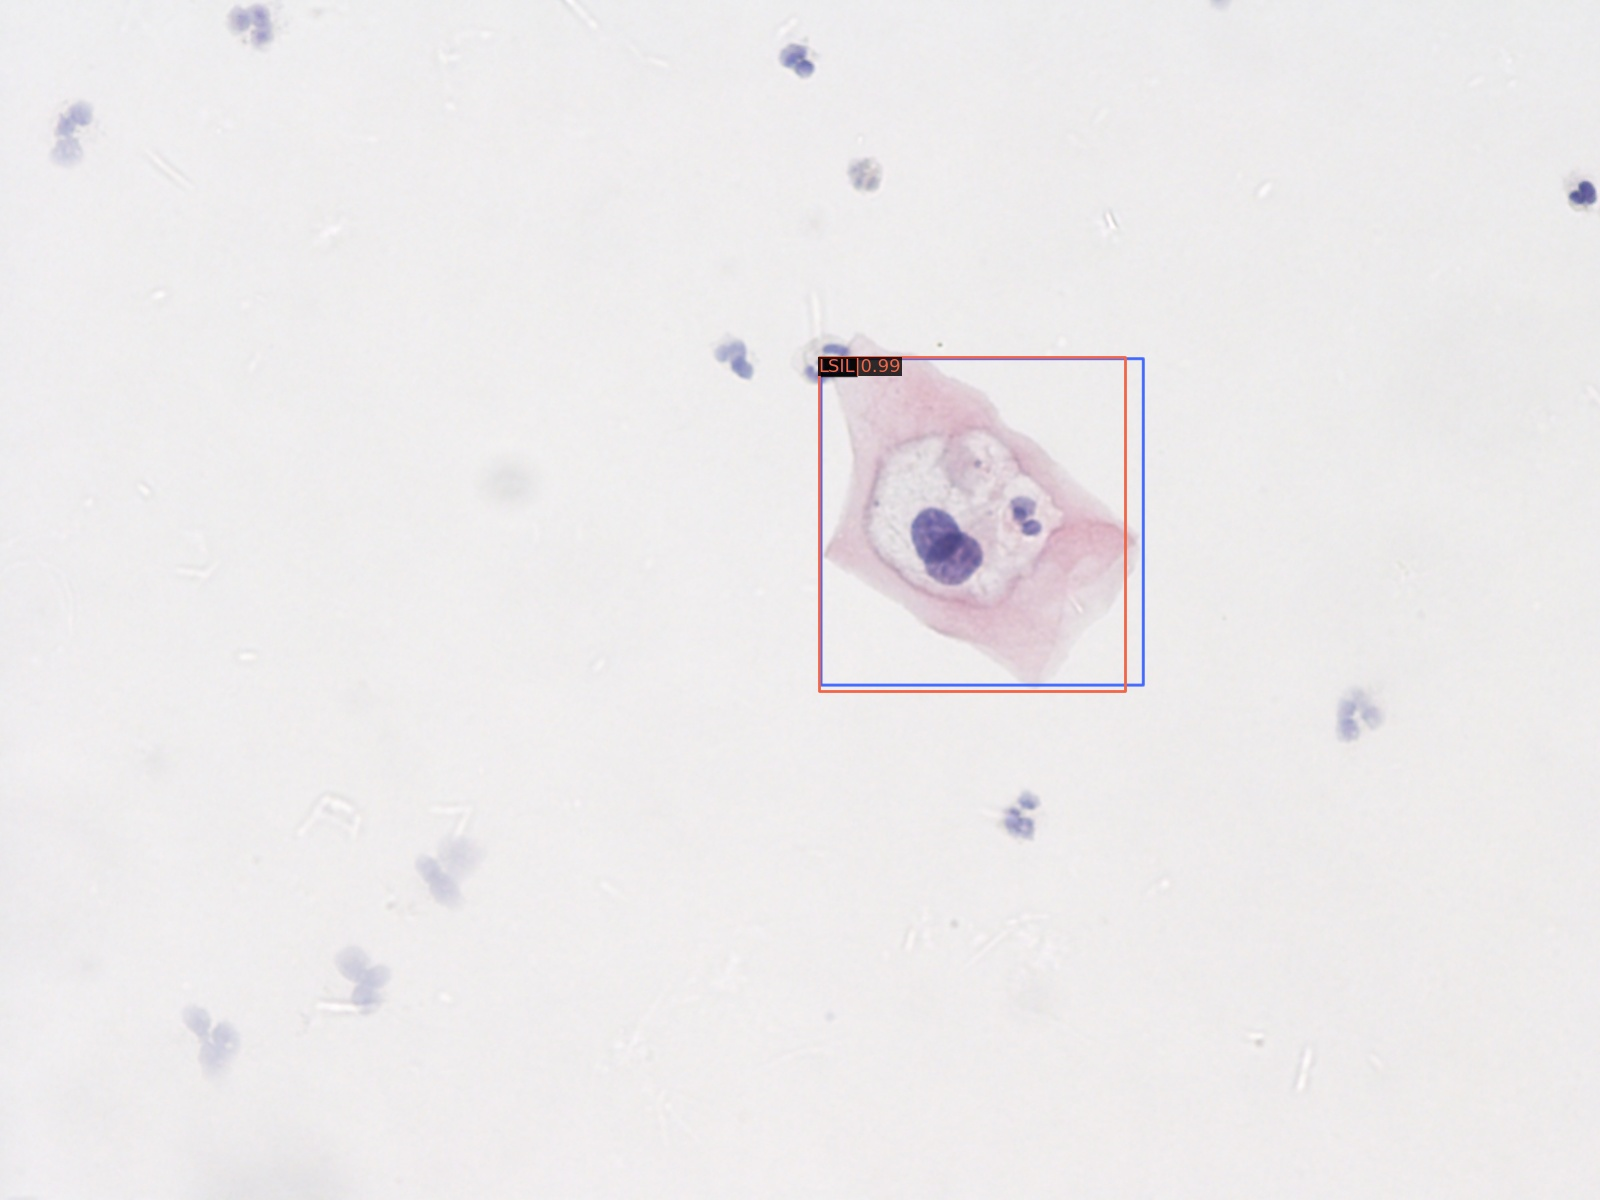
\includegraphics[width = .49\linewidth]{TCT/检测结果1.jpg}
    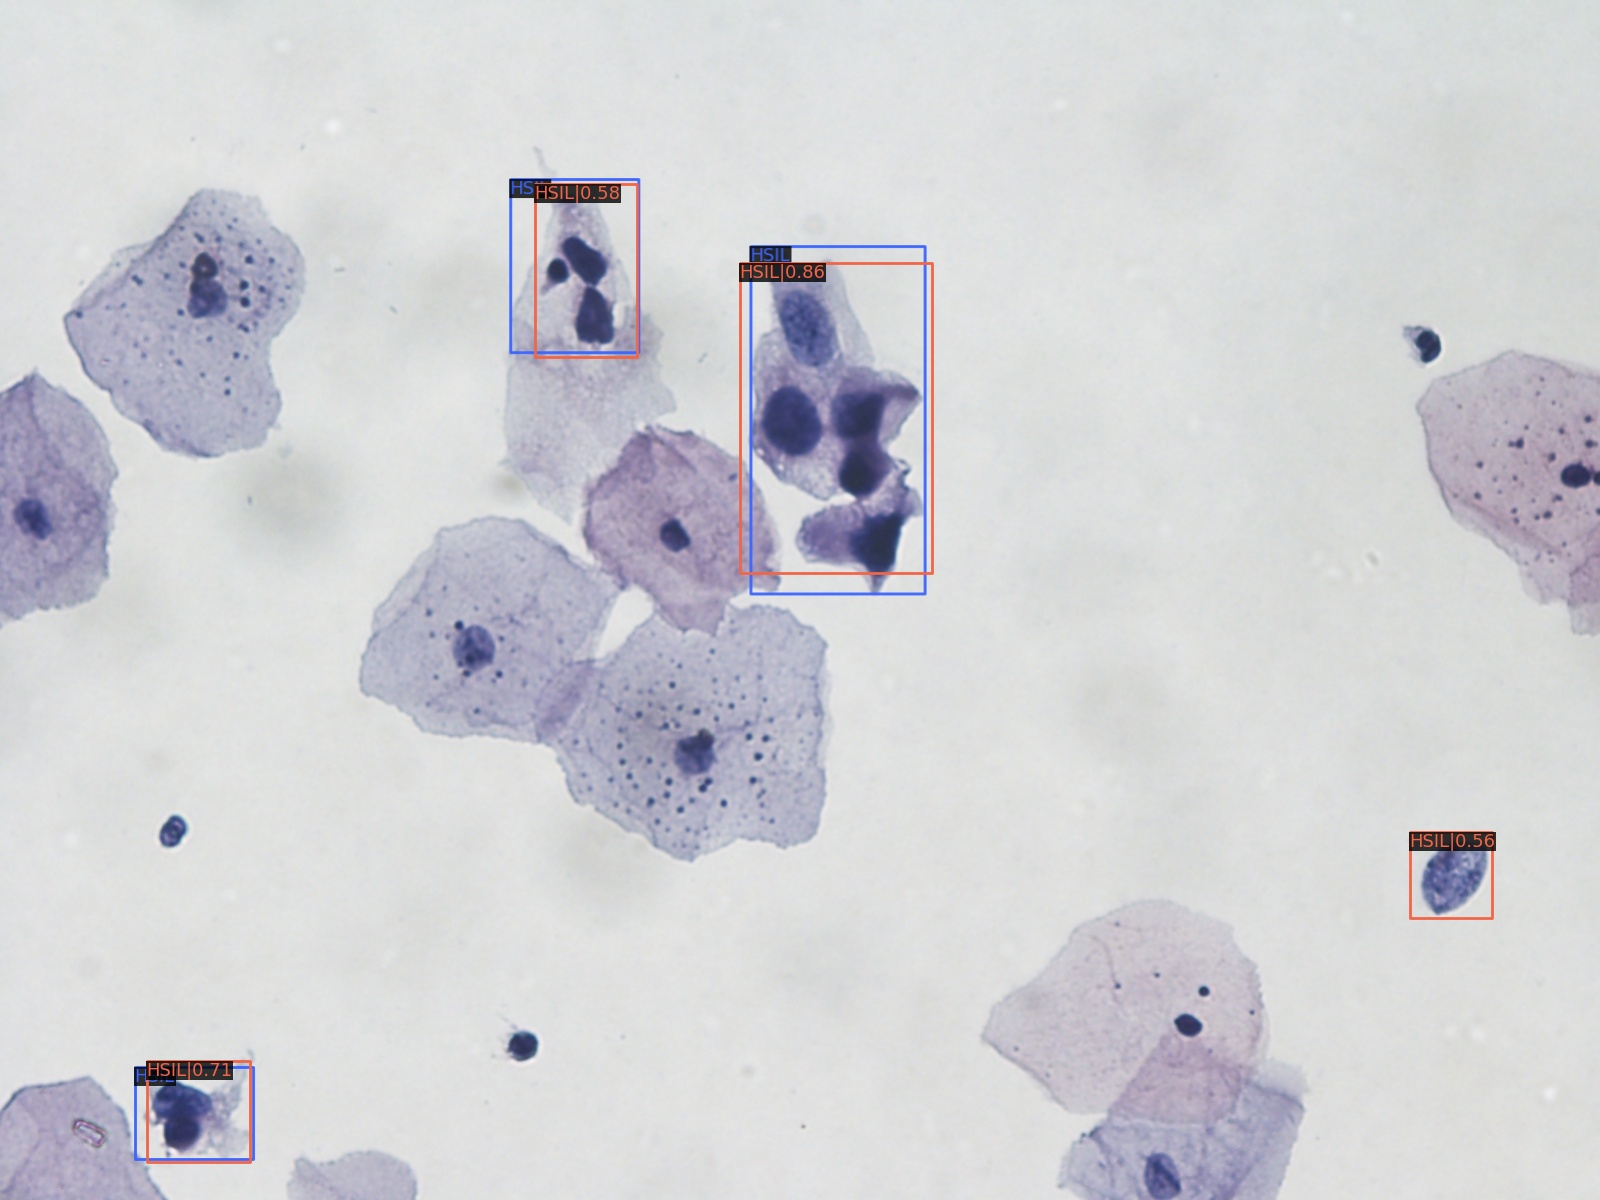
\includegraphics[width = .49\linewidth]{TCT/检测结果2.jpg}
    \caption{部分检测结果的可视化结果,其中橙色框是模型的预测结果,蓝色框是人工标注框。}
    \label{pic:检测结果可视化}
\end{figure}
\paragraph{基础模型的选择}
\par 在所有的基线模型中,Faster-RCNN模型有着最好的mAP50指标,仅次于Cascade R-CNN的mAP以及mAP75指标,也正是因此,我们才会选择Faster R-CNN作为基础,在其基础上完成后续工作。
\paragraph{与基线模型的检测性能比较}
\par 我们的模型与基线模型相比,尤其是Faster R-CNN相比,在mAP、mAP50以及mAP75等指标上都会有这一定的提升,这说明我们的方法对于增强模型检测病变细胞的能力是有帮助。
\paragraph{与宫颈病变细胞检测模型的检测性能比较}
\par 与Comparison detector等专为宫颈病变细胞检测任务优化的模型相比,我们的模型在各个指标上有着不小的优势。这说明我们的方法相较于其他宫颈病变细胞检测的方法也是有优势的。

\subsection{消融实验}
\subsubsection{任务分解}
\par 如章节\ref{sec:任务分解}所示,我们的模型首先使用两个单独的检测头完成单细胞与细胞簇的检测,因此,这前两个检测头的预测结果准确性十分重要。为此,我们设计了两组消融实验,第一个实验针对前两个检测头预测结果分正负样本时的iou阈值和前两个检测头损失函数的权重,第二个实验则探究RPN模块是否应该与检测头一样为单细胞和细胞簇两种检测任务分解为分离的两个RPN模块。

\paragraph{IOU阈值与损失权重消融实验}
\par 我们模型在异常细胞检测时使用的前两个检测头在计算loss时与Faster R-CNN一样需要首先将RPN模块提取出的目标区域提案按照与标注框的IOU大小和设定的阈值区分为正负样本,因此,在最终的检测头中,应当使用一个更高的IOU阈值。我们设置前两个检测头所使用的IOU阈值为0.5,而最终的检测头所使用的IOU阈值从0.5提高到0.6做消融实验。此外,由于我们的模型最终的输出结果完全来自最终的检测头,前两个检测头只是为最终的检测头提供一个比RPN模块更好的目标区域提案结果,因此,我们尝试降低前两个检测头的损失权重。我们设置最终的检测头的损失权重为1.0,前两个检测头的损失权重从1.0降低到0.5进行消融实验。结果如表\ref{tab:IOU阈值与损失权重消融实验}所示。IOU阈值从0.5提高到0.6可以在训练最终的检测头时,只留下更好的目标区域提案作为正样本,这会促进模型做出更准确的预测,进而提升模型的检测性能。而将前两个检测头的损失权重从1.0降低到0.5,可以让模型更关注最终检测头的预测结果,这也会有助于模型检测性能的提升。

\begin{table}[htbp]
    \centering
    \caption{IOU阈值与损失权重消融实验}
    \begin{tabular}{|c|c|c|c|c|c|}
        \hline
        IOU & 损失权重 & 验证集mAP50 & mAP  & mAP50 & mAP75 \\ \hline
        0.5 & 1.0      & 46.5        & 23.9 & 45.6  & 23.2  \\ \hline
        0.6 & 1.0      & 47.0        & 24.0 & 46.1  & 22.7  \\ \hline
        0.6 & 0.5      & 46.7        & 25.0 & 46.6  & 24.3  \\ \hline
    \end{tabular}
    \label{tab:IOU阈值与损失权重消融实验}
\end{table}

\paragraph{Multi-RPN}
\par 我们的模型使用两个单独的检测头完成单细胞与细胞簇的检测,通过分离检测头的方式让单细胞和细胞簇分别被不同的网络结构所捕捉并以此提升网络的检测性能,那么如果我们也将RPN分成两个不同的模块是不是可以进一步提升检测性能呢?为此,我们设计了Multi-RPN的消融实验,在实验中,我们尝试为不同的检测头使用不同的RPN网络,但是实验结果却说明RPN部分分离并不会带来明显的提升。
\par 这可能说明单细胞和细胞簇虽然有着较大的形态差异,但是其与背景之间的形态差异更大,虽然模型在为这些类别分类时可能会遇到困难,但是模型可以轻松地把它们与背景区分开来,因此,RPN即使不做分离依然可以很好的工作。

\begin{table}[htbp]
    \centering
    \caption{Multi RPN消融实验}
    \begin{tabular}{|c|c|c|c|c|}
        \hline
        Multi RPN  & 验证集mAP50 & mAP  & mAP50 & mAP75 \\ \hline
        \checkmark & 46.5        & 24.9 & 46.2  & 24.3  \\ \hline
        $\times$   & 46.7        & 25.0 & 46.6  & 24.3  \\ \hline
    \end{tabular}
\end{table}

\subsubsection{细胞对比}
\paragraph{正常细胞与异常细胞对比}
\par 我们的模型使用异常细胞特征与正常细胞特征相减的方式计算了异常细胞与正常细胞之间的差分特征,并将这一特征用于后续的检测任务。而且,我们还使用了存储机制,让模型在没有检测到正常细胞时,依然可以获取到在其他图像上检测到的正常细胞的特征,我们针对这两点做了消融实验。
\par 首先是有无存储器我们设置了两种不同的情况。在有存储器的情况下,模型如同我们之前所描述的那样工作。而没有储存器时,我们的模型则会在没有检测到正常细胞时直接使用全零的张量作为正常细胞的特征。其次是针对差分特征计算方式的消融实验,我们设计了差分、相加和融合三种不同的对比方式。差分特征的计算方法如我们之前所描述的一样,将正常细胞的特征复制到与异常细胞的特征相同的尺寸之后就直接使用异常细胞的特征减去正常细胞的特征即可,而相加的方式只是将异常细胞的特征减去正常细胞的特征改为加上正常细胞的特征,融合的方式则是指将正常细胞的特征复制到与异常细胞的特征相同尺寸之后,将两者拼接起来,然后让该特征图经过两个保持形状$1\times 1$卷积层并通过最后一个通道数只有原来一半的$1\times 1$卷积层使特征的通道数与拼接之前保持一致。
\par 实验结果如\autoref{tab:正常细胞与异常细胞对比方式消融实验}所示,特征差分的方式会明显优于特征融合的方式,而特征相加的方式优于仅仅改变了一个正负号,对于全卷积层来说只是学习到的权重相差一个正负号的区别,所以在检测性能表现上二者几乎相同。

\begin{table}[htbp]
    \centering
    \caption{正常细胞与异常细胞对比方式消融实验}
    \begin{tabular}{|c|c|c|c|c|c|}
        \hline
        有无存储器 & 对比方式 & 验证集mAP50 & mAP  & mAP50 & mAP75 \\ \hline
        有         & 差分     & 46.0        & 23.7 & 44.6  & 22.7  \\ \hline
        有         & 相加     & 45.3        & 23.9 & 44.3  & 24.0  \\ \hline
        有         & 融合     & 42.5        & 21.4 & 40.5  & 20.2  \\ \hline
        无         & 差分     & 46.6        & 20.1 & 38.8  & 19.3  \\ \hline
        无         & 相加     & 45.9        & 21.7 & 39.2  & 20.8  \\ \hline
        无         & 融合     & 41.7        & 20.7 & 39.8  & 20.0  \\ \hline
    \end{tabular}
    \label{tab:正常细胞与异常细胞对比方式消融实验}
\end{table}

\paragraph{异常细胞与异常细胞对比}
\par 我们的模型最终使用了分区版的关系特征计算方式,而这一计算过程会用到分区数量这一超参数。为此,我们设计了不同分区数量的消融实验。结果如\autoref{tab:异常细胞与异常细胞对比方式消融实验}所示,分区数对检测性能的影响不大,但由于关系计算模块所引入的参数量为$\text{特征维度}^2/\text{分区数量}$,因此,随着分区数逐渐接近特征维度的平方根,该模块所引入的参数量会逐渐减小。
\begin{table}[htbp]
    \centering
    \caption{异常细胞与异常细胞对比方式消融实验}
    \begin{tabular}{|c|c|c|c|c|}
        \hline
        分区数 & 验证集mAP50 & mAP  & mAP50 & mAP75 \\ \hline
        1      & 47.5        & 19.1 & 41.6  & 15.2  \\ \hline
        4      & 47.2        & 19.0 & 40.9  & 14.7  \\ \hline
        8      & 48.0        & 19.3 & 42.3  & 14.3  \\ \hline
        16     & 47.7        & 19.6 & 41.8  & 15.3  \\ \hline
        32     & 48.0        & 20.4 & 42.3  & 17.0  \\ \hline
    \end{tabular}
    \label{tab:异常细胞与异常细胞对比方式消融实验}
\end{table}

\paragraph{对比关系与检测头}
\par 我们的模型所使用的会计算异常细胞与异常细胞之间的关系特征,以及正常细胞与异常细胞之间的差分特征等。而我们的模型在异常细胞检测部分又有着三个检测头,那么我们应该在三个检测头中都加入细胞对比的方法吗?为此,我们设计了三个检测头都加入细胞对比和只有最终的检测头加入细胞对比的消融实验。结果如表\ref{tab:细胞对比消融实验}所示,我们只需要在最终的检测头中加入细胞对比的方法即可获得性能提升。在三个检测头中都加入细胞对比的方法反而会使模型的检测性能下降,这可能是因为,加入细胞对比的方法会引入不少的参数,三个检测头都加入会使模型参数量过多,在算力有限的条件下不易训练到一个更好的结果。

\begin{table}[htbp]
    \centering
    \caption{细胞对比消融实验}
    \begin{tabular}{|c|c|c|c|c|}
        \hline
        对比Head   & 验证集mAP50 & mAP  & mAP50 & mAP75 \\ \hline
        仅TCT Head & 49.3        & 24.9 & 47.6  & 24.3  \\ \hline
        三个 Head  & 47.8        & 24.7 & 47.3  & 24.4  \\ \hline
    \end{tabular}
    \label{tab:细胞对比消融实验}
\end{table}

\subsection{正常细胞半监督检测}
\par 如章节\ref{半监督学习与伪标签的生成}中提到的,我们通过使用不同比例的正常细胞标注启动半监督的学习机制以探究该机制对正常细胞标注数量的最低需求。在该实验中,我们将训练集中的正常细胞只保留设定的比例用于训练,之后通过验证集筛选出最优模型,最后将模型在测试集上的预测结果和测试集上全部的标注结果计算mAP指标作为模型的最终成绩,结果如表\ref{tab:正常细胞半监督检测}所示。
\par 如果我们保留很低比例(比如,1\%)的标注框,那么随着迭代轮数的不断提升,我们的模型可以越来越好的学习到如何检测正常细胞并会有一个比较明显的检测性能提升。而如果我们保留较低比率的正常细胞标注框(比如,3\%到10\%)的标注框,那么随着迭代轮数的不断提升,我们的模型刚开始会有一个比较明显的检测性能提升,但随后检测指标反而会下降。这一点在我们保留较高比例的正常细胞标注框(比如,25\%及以上)时尤为明显,这是因为我们本来的正常细胞标注框就是部分标注,我们仅仅标注出了图片中极少量的正常细胞标注框,典型的一张图片中可能会有十几到几十个正常细胞,但是我们的标注可能只会标出一到三个正常细胞,因此,随着模型的检测性能和泛化性能逐渐提升,模型会越来越多地检测到未标注的正常细胞,而这些检测结果都会在计算指标时被当作假阳性而导致指标下降。为了解决这个问题,我们只能通过人工查看模型标注结果的方式来进行评价模型的检测性能。经过我们的人工判断之后,我们可以认为当我们保留5\%及以上也即一百五十个正常细胞标注框及以上时,模型通过这种机制几乎可以在第一轮或第二轮迭代中学会检测正常细胞,其检测结果已经完全足以作为正常细胞特征用在我们的模型中。当我们保留3\%也即九十个正常细胞标注框左右时,模型可以通过该机制在三到四轮时学会检测正常细胞,而如果我们仅保留1\%也即三十个正常细胞标注框左右时,模型需要五轮及以上才可以学会检测正常细胞。
\par 由此,我们可以认为我们的半监督学习机制只需要一百五十个正常细胞标注即可很快地完成正常细胞检测任务的学习,而我们推荐至少在拥有一百个左右的正常细胞标注时再通过该机制让模型学习捕捉正常细胞,更少的标注可能会带来检测性能的下降。

\begin{table}[htbp]
    \centering
    \caption{正常细胞半监督学习结果}
    \begin{tabular}{|c|c|c|c|c|c|}
        \hline
        \diagbox{倍率}{mAP50}{轮数} & 1    & 2    & 3    & 4    & 5    \\ \hline
        1\%                         & 11.9 & 18.2 & 16.3 & 19.0 & 21.0 \\ \hline
        3\%                         & 19.6 & 25.7 & 23.3 & 23.2 & 19.1 \\ \hline
        5\%                         & 26.5 & 30.6 & 28.5 & 27.3 & 26.7 \\ \hline
        10\%                        & 27.9 & 27.4 & 28.4 & 26.4 & 24.5 \\ \hline
        25\%                        & 32.1 & 31.9 & 29.8 & 25.1 &      \\ \hline
        50\%                        & 35.0 & 34.2 & 33.9 & 29.6 &      \\ \hline
        75\%                        & 36.1 & 35.8 & 33.4 & 32.1 &      \\ \hline
        100\%                       & 38.8 & 35.7 & 32.7 & 35.3 &      \\ \hline
    \end{tabular}
    \label{tab:正常细胞半监督检测}
\end{table}
\par 部分正常细胞检测结果的可视化如图\ref{pic:正常细胞检测结果可视化}所示。在选用IOU阈值为0.5时,经过适当轮数的训练之后模型检测到的正常细胞框都是对的,而且都可以检测出足量的正常细胞用于后续的检测任务。
\begin{figure}[htb]
    \centering
    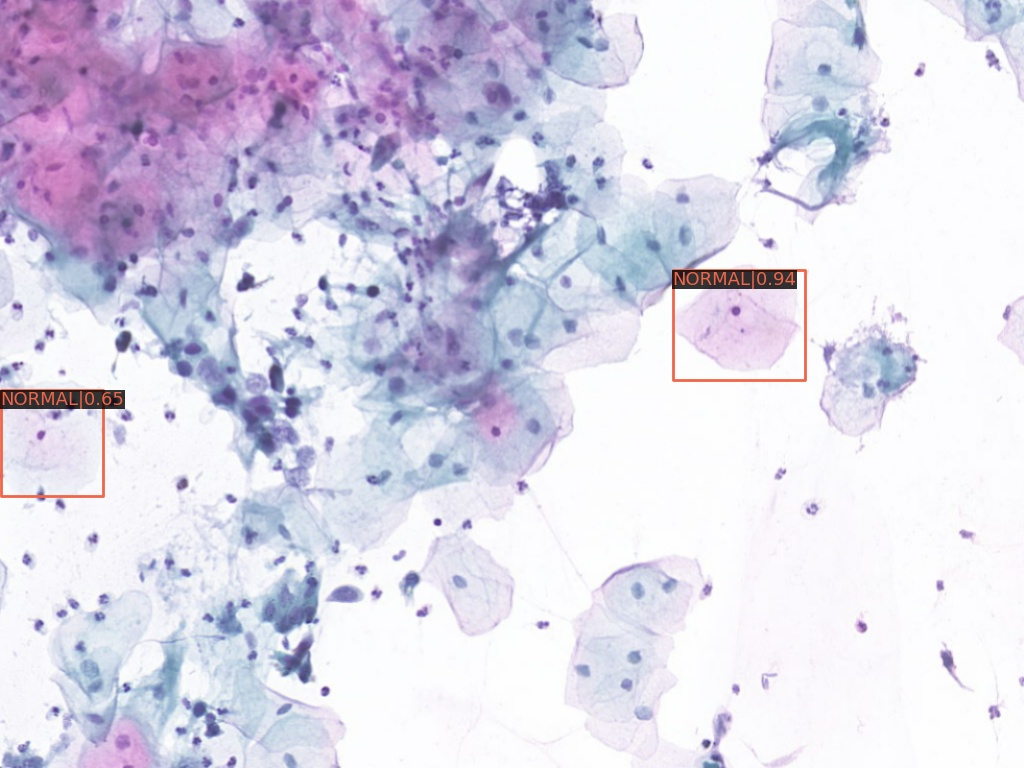
\includegraphics[width = .49\linewidth]{TCT/正常细胞检测结果1.jpg}
    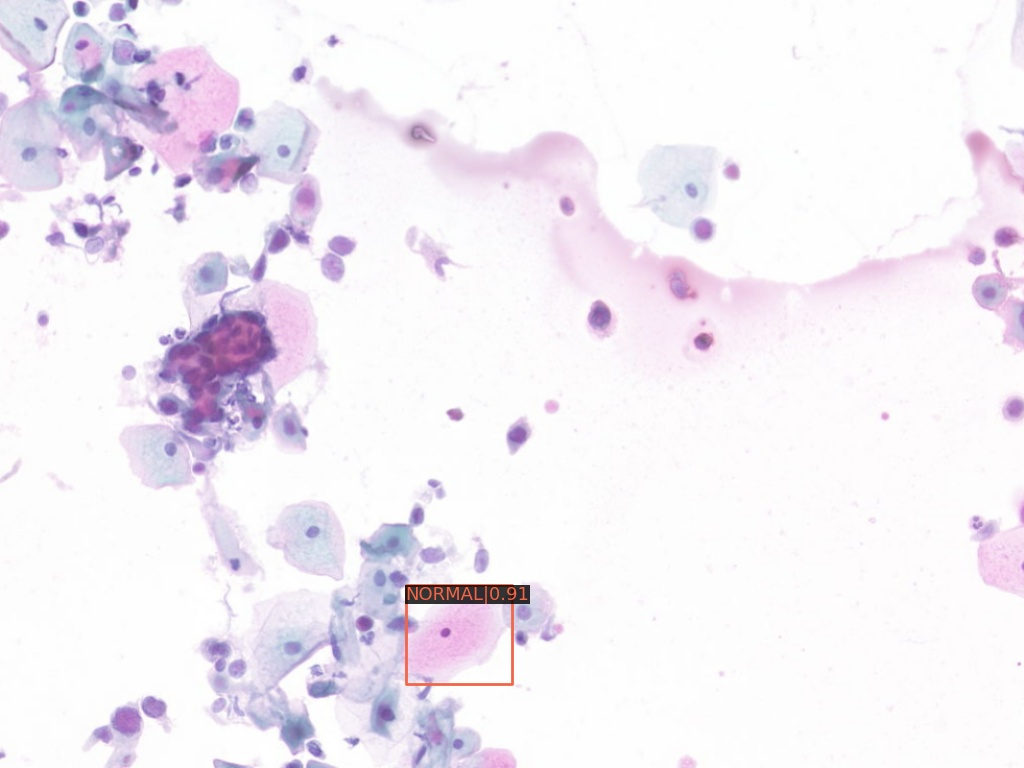
\includegraphics[width = .49\linewidth]{TCT/正常细胞检测结果2.jpg}
    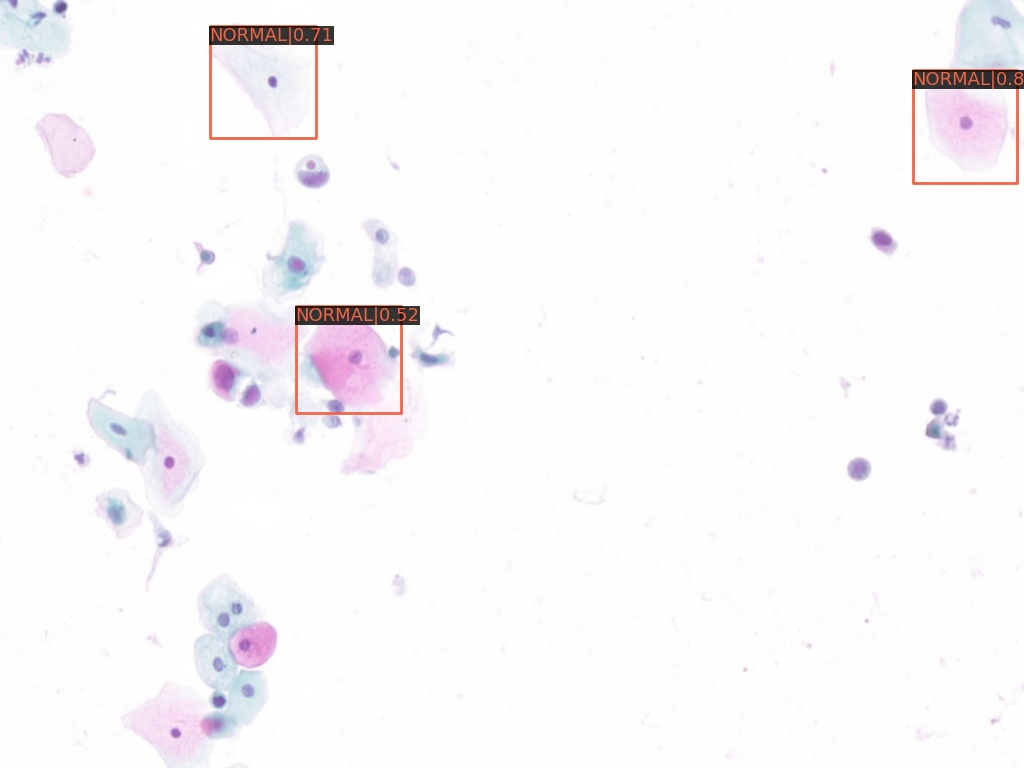
\includegraphics[width = .49\linewidth]{TCT/正常细胞检测结果3.jpg}
    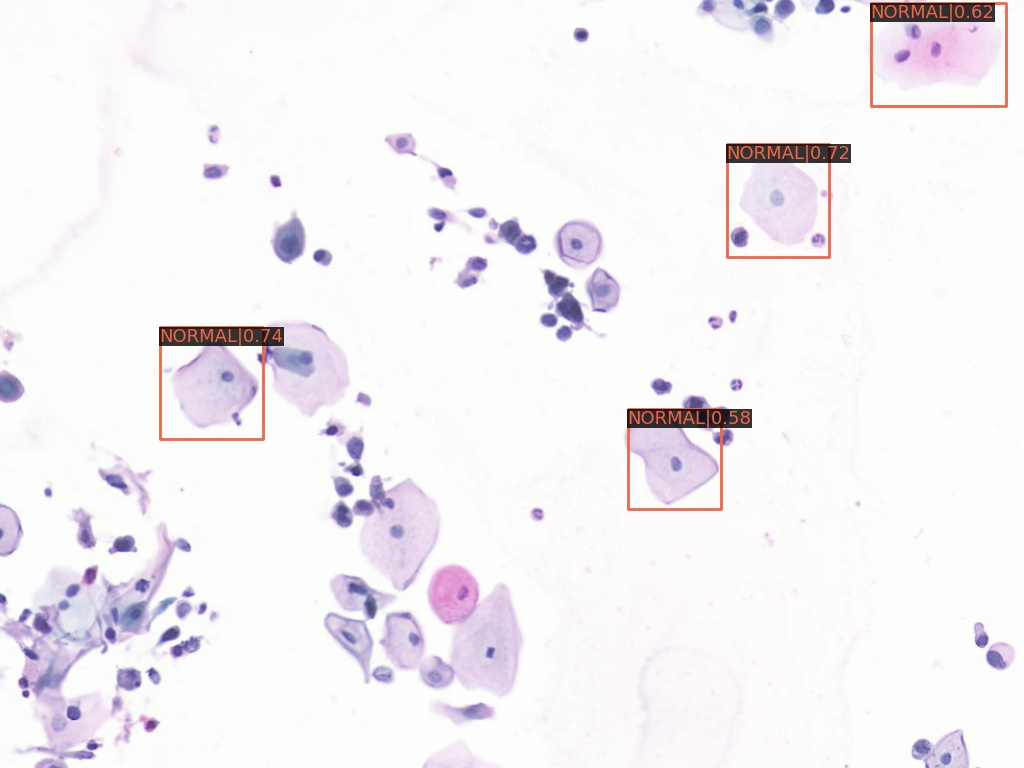
\includegraphics[width = .49\linewidth]{TCT/正常细胞检测结果4.jpg}
    \caption{部分正常细胞检测结果的可视化结果}
    \label{pic:正常细胞检测结果可视化}
\end{figure}

\clearpage

\section{总结与展望}

\subsection{结论}
\par 如章节\ref{sec:计算机辅助检查面临的问题}所示,使用计算机辅助宫颈病变细胞检测领域面临着单细胞与细胞簇的形态差异、放大倍率不一致等问题,本文基于Faster R-CNN网络,通过加入任务分解机制解决了模型在面对单细胞与细胞簇标注框的形态差异与语义差异时产生的特征冲突等问题,并通过细胞对比机制,缓解了TCT图片放大倍率不一致带来的细胞特征提取以及类别判断的困难,还利用半监督学习的方法,让模型仅依靠少量的正常细胞标注就可以学会捕捉正常细胞的特征并将其提取出来用于细胞对比过程。我们设计的这一网络在相较于Faster R-CNN等基线模型以及其他针对宫颈病变细胞检测任务优化的模型有一定检测性能和检测准确率上的提升。说明我们所设计的相关模块与方法对宫颈病变细胞检测这一任务是有所帮助的。

\subsection{创新点}
\par 本文的主要创新在于使用了任务分解和细胞对比两大机制以及通过半监督学习的方法让模型可以在极少量正常细胞标注的情况下学会检测正常细胞,并提取其特征。

\paragraph{任务分解}
\par 在TCT图片中,病变细胞的标注框往往包含两类:只含有一个细胞和含有两个及以上细胞的标注框,这两类标注框在形态和语义上有着很大的区别,但是现有的宫颈病变细胞检测工作往往直接使用传统的自然图像领域的目标检测方法,而没有针对TCT图片中的这个特点做出相应优化,本文提出的任务分解机制专门针对TCT图片的这一特点设计了专门的网络模块,可以让网络更好的捕捉病变细胞的形态特征并可以缓解网络学习过程中遇到的特征冲突等问题。

\paragraph{细胞对比}
\par TCT的图片都是经由显微镜放大得到的,其绝对大小没有意义,只有相对大小才有意义,而传统的自然图像领域的目标检测算法往往使用FPN层在处理图像,又在检测头中没有目标区域提案相互参照的部分,因此,对于TCT图片中某些形态特征相近而尺寸相差较大的目标很难做出正确的区分。本文针对这一问题提出细胞对比机制,通过正常细胞与异常细胞的对比以及异常细胞与异常细胞之间的相互对比加强了模型对于上述问题的解决能力,并进而获得了检测性能的提升。

\paragraph{半监督正常细胞检测}
\par 在实际的使用过程中和临床实践过程中,医生往往只会标注病变细胞并不会注明正常细胞的位置,因此,我们通过引入半监督学习的方法让模型在仅有极少量正常细胞标注的情况下依然可以学会检测正常细胞并提取出其特征用于细胞对比。这为我们设计的细胞对比部分的正常运行提供了保障。

\subsection{研究展望}
\par 本文使用了任务分解和细胞对比两大机制来完成宫颈病变细胞检测的任务,其中,我们通过半监督学习的方法让模型可以在极少量正常细胞标注的情况下学会检测正常细胞,并提取其特征用于细胞对比部分,但是,任务分解部分需要我们手工的将所有的标注框区分为Single和Multi两大类,无法让计算机自动地完成相应工作,因此,如何通过进一步引入半监督等机制让模型可以自动地完成任务分解中标注框分解的工作是一个进一步研究的方向,这将能够极大减少本文方法在使用过程中所需要的工作量。此外,本文在对比正常细胞与异常细胞时只是简单地做了减法,虽然该方法被实验证明比使用卷积层融合的方法更加有效,但是过于简单了,如何设计一定的模块进一步提升细胞对比对模型捕捉异常细胞特征的贡献是值得进一步探究的。
